\chapter{Estudo de Caso}
\label{cap-case-study}

%

Neste capítulo será apresentada a utilização dos Cenários de Decisões em projetos reais, com o principal objetivo de demonstrar a reprodução de cenários em ambientes de tomada de decisão. Assim, este Capítulo é destinado ao Estudo de Caso de utilização das ferramentas Mezuro e DWing para observação de Cenários de Decisões em projetos de software.

Para tanto, será apresentada a avaliação de três projetos de softwares livres em C++. Além disso, iremos explicar os passos necessários para reproduzir a estrutura de cenários nos dois ambientes de tomadas de decisões abordados nesta monografia. Assim, será apresentado as principais evoluções e adaptação de cada ferramenta e os detalhes específicos da observação de cada cenário.

O método de execução desses estudos de casos é apresentado na Figura~\ref{method}. Nesta figura são descritos os passos necessários para reproduzir cenários em ferramentas que apoiam a tomada de decisões baseados em métricas de software que, no contexto desta monografia, consiste no Mezuro e DWing.

\graphicspath{{figuras/}}
\begin{figure}[h]
\centering
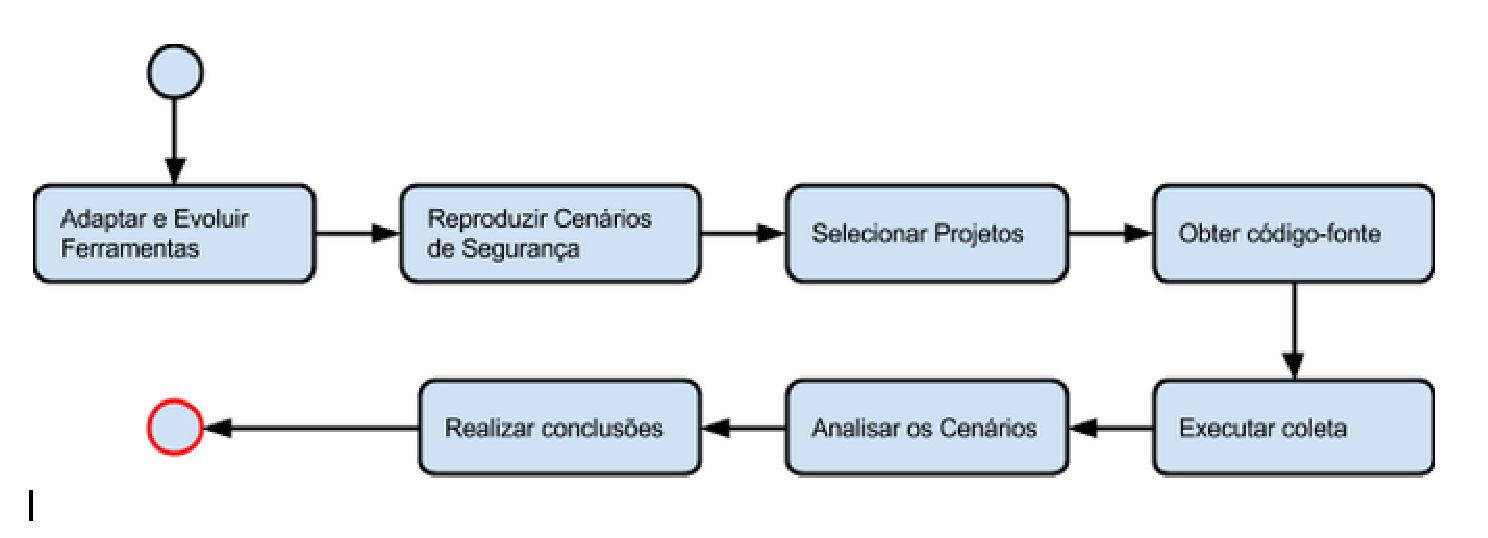
\includegraphics[width=1.0\textwidth]{fluxograma}
\caption{Método para execução dos estudos de casos.}
\label{method}
\end{figure}

Os passos da Figura~\ref{method} são melhor descritos a seguir:

\begin{enumerate}
\item \textbf{Adaptar e Evoluir Ferramentas} - Este passo consiste em evoluir as estruturas, modelos, componentes e camada de apresentação das ferramentas que serão utilizadas com o objetivo de melhor suportar a utilização de Cenários de Decisão.
\item \textbf{Reproduzir Cenários} - Uma vez que as ferramentas utilizadas já suportam a reprodução de Cenários, deve-se utilizar dessa estrutura para definir cenários reais para avaliação de projetos de software. No contexto dessa monografia, esse passo consiste em reproduzir os Cenários de Segurança criados no Mezuro e no DWing.
\item \textbf{Selecionar Projetos} - Esta etapa consiste em definir quais projetos serão avaliados a partir dos cenários definidos e pode ser executada independente das ferramentas de tomada de decisão, variando de acordo com os objetivos de utilização dos Cenários.
\item \textbf{Obter Código-Fonte} - Uma vez selecionados os projetos, o próximo passo é obter o código-fonte referente aos projetos escolhidos. Algumas ferramentas. como o Mezuro, já possuem bom suporte para automatizar esse passo.
\item \textbf{Executar Coleta} - Esta etapa consiste na obtenção dos valores de métricas dos códigos-fontes dos projetos selecionados que deve ser automatizado. A saída desta etapa deverá ser processada pelas ferramentas trabalhadas para proporcionar a análise dos projetos. O esforço nessa etapa deve-se reduzir a coletar somente as métricas necessárias para composição dos Cenários de Decisão utilizados.
\item \textbf{Analisar Cenários} - A partir dos resultados obtidos, deve-se utilizar os Cenários de Decisão para observar as características do estado atual do projeto analisado. No contexto desse trabalho, esta etapa consiste em analisar quais os principais módulos oferecem riscos de segurança ao software.
\item \textbf{Realizar Conclusões} - Esta etapa final consiste em realizar ações a partir da compreensão dos Cenários observados, seja para fins de estudos ou para fins de desenvolvimento do software. 
\end{enumerate}


Estes passos metodológicos devem ser reproduzidos para cada ferramenta utilizada, sendo que uma vez que uma ferramenta já suporta adequadamente a observação de Cenários de Decisão, os passos 1 e 2 não precisam ser repetidos para análise de novos projetos.


\section{Criação dos Cenários do Mezuro}
\label{mezuro-cenarios}

O Mezuro é uma plataforma livre para monitoramento de código-fonte que busca auxiliar em vários problemas relacionados à utilização de métrica, visando ser uma interface que permita, de forma flexível, a extração e análise de métricas estáticas de código-fonte, licensiado como AGPLv3\footnote{\url{http://www.gnu.org/licenses/agpl-3.0.html}} \cite{manzo2014}. O Mezuro é uma plataforma concebida através do amadurecimento de diversas ferramentas, inicializada através do projeto Qualipso\footnote{Quality Platform for Open Source: \url{http://qualipso.icmc.usp.br/}}. Dentre estas ferramentas, destaca-se o Analizo\footnote{\url{http://analizo.org/}}, uma das ferramentas utilizadas pelo Mezuro para extração de métricas de código-fonte em C/C++ e Java.

A arquitetura do Mezuro atual é composta por vários serviços. Essa arquitetura está evoluindo para uma arquitetura de composição de cinco serviços que se resumem em:

\begin{itemize}
\item \textbf{Prezento}: Camada de apresentação da plataforma desenvolvida em Ruby on Rails.

\item \textbf{Kalibro Gatekeeper}: Serviço que faz a intermediação e orquestração das outras camadas com o Prezento.

\item \textbf{Kalibro Processor}: Serviço que centraliza o processamento de métricas de projetos.

\item \textbf{Kalibro Project}: Serviço que realiza todo processamento relacionado aos projetos analisados.

\item \textbf{Kalibro Configuration}: Serviço responsável pelo processamento de configurações.
\end{itemize}

Uma explicação mais detalhada desta arquitetura e de cada serviço pode ser obtida no Apêndice \ref{Att:mezuro}.

Três destes serviços agregam conceitos fundamentais dentro da plataforma, que também serão muito importantes para a representação de cenários dentro da plataforma. 

O Kalibro Project contempla o conceito de projeto, onde são mantidos os códigos e informações de projetos que serão analisados. Atualmente, o Mezuro realiza o download de projetos que estão em repositórios GIT ou SVN. Além disso, o Mezuro pode monitorar projetos em C, C++ e Java uma vez que utiliza o Analizo como seu principal extrator de métricas. Entretanto, com a evolução da plataforma, pretende-se acoplar novos extratores na ferramenta para outras linguagens de programação.

O Kalibro Configuration contempla o conceito de configuração que é um conjunto de métricas e parâmetros que podem ser utilizadas para a avaliação de um projeto. Uma configuração consiste, portanto, na composição de métricas cujos valores de referência são flexíveis e podem ser determinados separadamente para cada configuração criada. Associado ao conceito de configuração, está a criação de intervalos qualitativos associado a valores de métricas. Esta característica é muito importante para a utilização das métricas, uma vez que abstraem a interpretação direta dos valores obtidos para definições mais simples como bom, regular e ruim. Assim, tem-se a flexibilidade de ter parâmetros que variam de acordo com a linguagem, natureza do software, dentre outras coisas, apenas pela criação de diferentes configurações.

O Kalibro Processor contempla o módulo de extração e processamento de métricas de código-fonte. Para que esse processamento seja realizado, o Kalibro Processor utiliza uma ou mais ferramentas de extração de métricas, como mencionado anteriormente. Assim, obtem-se a partir da análise estática do código-fonte um conjunto de métricas nativas que podem ser compostas para formular métricas mais complexas e de maior valor interpretativo. Dentro do Mezuro, esta abordagem é realizada através da criação de métricas compostas as quais serão muito importantes para a definição de Cenários de Decisões.


explicar primeiro como o Mezuro foi utilizado para suportar os Cenários, o que foi adaptado e melhorado para melhor suportar cenários, etc.

Depois deve-se mostrar a estrutura de cada cenário dentro da ferramenta (scripts e configuração)

\section{Criação dos Cenários do DWing}
\label{dw-cenarios}

Como o nome sugere, \emph{Data Warehouse} (DW), em português, significa armazém de dados. Segundo Inmon (\citeyear{inmon2002}) um \emph{Data Warehouse} é uma coleção de dados de uma coorporação que tem como objetivo dar suporte a tomada de decisão. 
%
O DW possibilita a análise de grandes volumes de dados, fazendo com que ele seja o núcleo de muitas soluções de \emph{Business intelligence} (BI)
%
\footnote{\emph{Business intelligence} é o processo de coleta, organização, análise, compartilhamento e monitoramento de informações, oferencendo suporte a gestão de negócios}. 
%

Neste trabalho procuramos desenvolver mecanismos que nos permitam monitorar e analisar o código fonte através de métricas de forma automatizada e que nos auxilie na tomada de decisão de refatorar ou não refatorar determinadas partes do código. 
%
Nesse sentido, foram encontrados alguns trabalhos na literatura que utilizaram o DW para monitorar métricas de processos e produtos de software \cite{Folleco2007} \cite{Silveira2010}\cite{mazuco2011}. Dentre estes, o que se destaca é o trabalho de  \cite{Silveira2010} que propõe um processo automatizado de extração e carga em um repositório central de métricas de qualidade de software. O autor também oferece suporte a monitoração dos projetos utilizando a técnica EVA e a análise da qualidade interna do software para o auxilio a tomada de decisões sobre os projetos analisados. O trabalho de \cite{rego2014} propõe um ambiente de DWing para o monitoramento de métricas e cenários relacionados a qualidade de software. Este ultimo foi usado como ponto de partida para criação e evolução do modelo dimensional do ambiente de DWing.

% 
O fato de o DW oferecer um alto poder de análise e poder tratar uma grande quantidade de dados nos faz ter uma espectativa de que esse ambiente pode ser uma solução mais completa em termos de monitoramento e auxílio na tomada de decisão. Entretanto, temos a hipótese de que o DW seja uma solução mais adequada para o uso por gerentes ou líderes de projeto, diferente do Mezuro que poderia ser melhor utilizado no uso cotidiano dos desenvolvedores. Mas essas são apenas hipóteses que serão validadas com a real comparação entre os dois ambientes implementados.

O conjunto de ferramentas de manipulação de dados, desde sua extração até a visualização para o apoio a consultas e tomada de decisição é denominado de \emph{Data Warehousing} (DWing). Portanto,  \emph{DWing} não são as tecnologias em si envolvidas e sim uma arquitetura que requer o suporte de diferentes tipos de tecnologias \cite{inmon2002}.  As principais tecnologias envolvidas em um ambiente de \emph{DWing} são:


\begin{itemize}
\item SGBDS – Gerenciadores de bases de dados
\item Sistemas de conversão e transformação de dados (ferramentas de ETL)
\item Tecnologias cliente e servidor para dar acesso aos dados a múltiplos clientes
\item Ferramentas de análise e geração de relatórios.
\end{itemize}


Kimball (\citeyear{kimball2002}) define os componentes básicos de um ambiente de \emph{DWing} conforme a Figura \ref{componentesdw}.

 \begin{figure}[!htb]
 	\centering
 		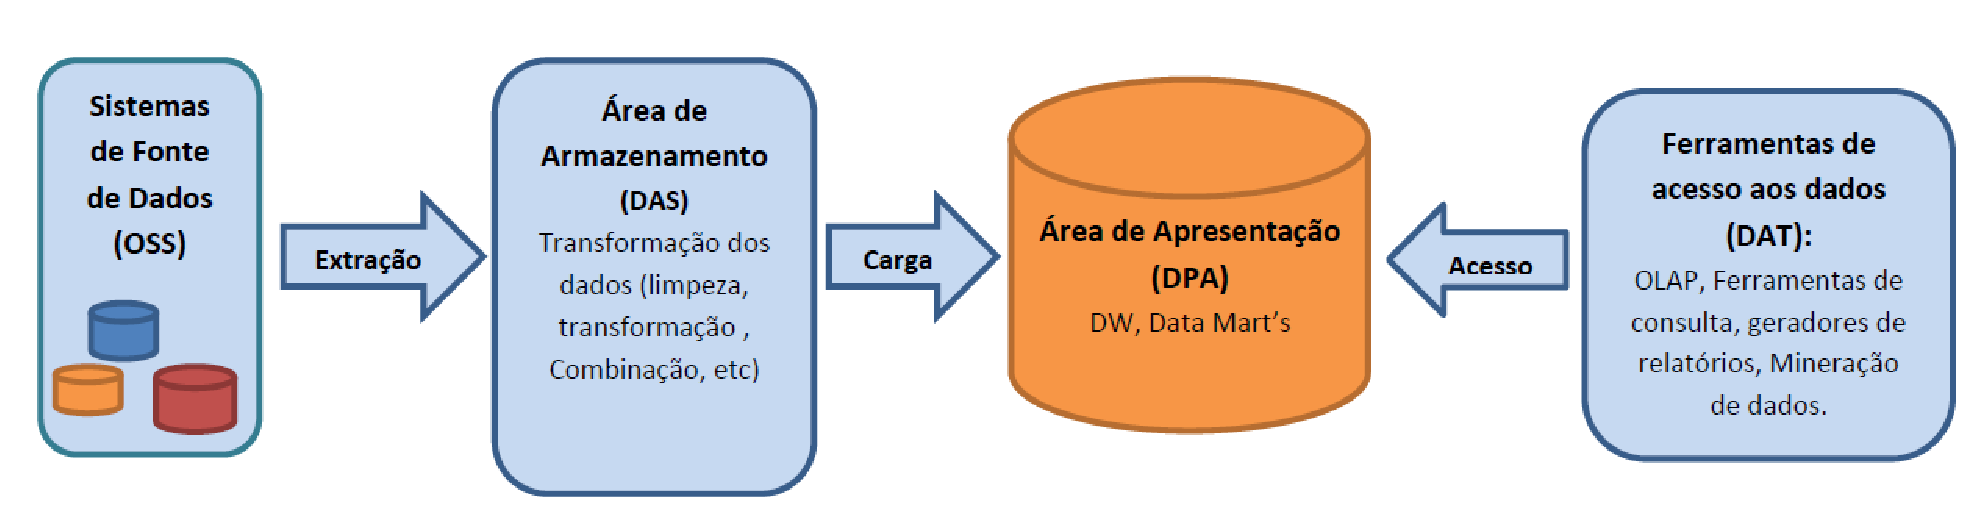
\includegraphics[scale=0.5]{figuras/componentesDW}
 		\caption{Componentes de um \emph{DWing}. Adaptação de \cite{kimball2002}}.
 		\label{componentesdw}
 \end{figure}


%TODO: ver se concorda com o fato de não termos subseções aqui
% a figura acima estava sem explicação/interpretação "explicita"
 A extração dos dados que irão compor o DW é feita de fonte de dados de sistemas, podendo ser de um ou vários sistemas relacionados. Esses dados são tratados na DSA, onde podem ser combinados, limpados ou transformados, tornado-os mais consistentes para que possam então ser amazenados na DPA, que seriam o DW ou \emph{Data Mart's}
 %
 \footnote{\emph{Data Mart} é um subconjunto de dados de um DW. Foca em uma ou mais áreas específicas \cite{kimball2002}}. 
 %
 As ferramentas de acesso são as responsáveis pela análise dos dados, podendo realizar consultas, gerar relatórios entre outros mecanismos de visualização.

Dado cada componente que compõe um ambiente de DWing, a seguir iremos detalhar algumas características de cada um deles já aplicando a criação do ambiente de DWing construido neste trabalho.

\subsection{Sistemas de fonte de Dados}

Os Sistemas de Fonte de Dados são os sistemas que irão fornecer os dados para o ambiente de DWing. No contexto dessa monografia, queremos colher métricas de software para fazer a análise e identificar a existência dos cenários definidos. Dessa forma, o Analizo é considerado um sistema de fonte de dados, pois fornece um relatório CSV com os valores das métricas de um projeto. O Analizo fornece tanto as métricas de qualidade quanto as métricas de vulnerabilidades utilizadas nos cenários propostos. 

Porém, foi identificado um problema com o Analizo de forma com que, para projetos maiores, ele não consegue gerar as métricas de vulnerabilidade. Esse problema será explicado mais adiante na seção (\ref{data-colect}). Mas uma característica de um ambiente de DWing é ser integrado. Isso quer dizer que um DWing é capaz de integrar dados de diversas fontes. Dessa forma, foi utilizado o clang-static-analyzer para coleta das métricas de vulnerabilidades usadas nos cenários propostos.


\subsection{Area de Apresentação - DPA}

Explicar modelo, maria DB, msqlworkbench


\subsection{Área de Armazenamento - DSA}

explicar uso do PDI,ETL, nao entrar em muitos detalhes do ETL, porém falar sobre os passos onde foram feitas as identificações dos cenários


\subsection{Ferramentas de Acesso aos dados - DAT}

Explicar o uso do BI server, como visualizar os cenários, mostrar a criação das hierarquias de agregação





explicar primeiro como o DW foi utilizado para suportar os Cenários, o que foi adaptado e melhorado para melhor suportar cenários, etc.

Depois deve-se mostrar a estrutura de cada cenário dentro da ferramenta (scripts e configuração)

\section{Projetos analisados}
\label{cap-projects}

Nesta monografia definimos a técnica de Cenários de Decisão e propomos um conjunto de cenários para tomada de decisão sobre a segurança do software, seja a partir da utilização de métricas de \emph{design} ou através de métricas de vulnerabilidades. Para apresentar como estes cenários podem ser utilizados, foram analisados três softwares livres. 

Como discutido no Seção \ref{cap-cenarios-sec-definicaocenarios} do Capítulo de Cenários, nos restringimos a apenas projetos escritos em C++. A seguir é feita uma pequena introdução à cada um dos projetos escolhidos.

\subsection{GNU Octave}
\label{section-octave}

O GNU Octave é um projeto desenvolvido em C++ que consiste em uma linguagem interpretada de alto nível destinada à computação matemática distribuída através da licença GNU General Public License \footnote{\url{http://www.gnu.org/copyleft/gpl.html}}. Ele possui uma interface baseada em linha de comando para a solução de problemas matemáticas lineares e não lineares, assim como possibilita a execução de experimentos numéricos. Além disso, também provê um conjunto extensivo de ferramentas para geração de gráficos, visualização e manipulação de dados.

Outras informações específicas sobre o projeto GNU Octave podem ser obtidas através da documentação oficial do projeto, disponível na página \url{https://www.gnu.org/software/octave/}.

O código fonte do projeto está disponível na página \url{ftp://ftp.gnu.org/gnu/octave}. Lá, além da versão atual, podemos ter acesso ao código de releases anteriores.

Este projeto será analisado tanto através do Mezuro quanto através do DWing.


==== MOSTRAR OS CENÀRIOS EM CADA FERRAMENTA ====


\subsection{Athom Shell}
\label{section-athom}

O Athom Shell é um framework desenvolvido em C++ que permite escrever aplicações \emph{desktop} multi-plataforma através de JavaScript, HTML e CSS. Esse framework é baseado em node.js\footnote{\url{http://nodejs.org/}} e no Chromium e é usada no editor de texto Athom\footnote{\url{https://atom.io/}}. Esse projeto é distribuído através da licença MIT\footnote{\url{http://opensource.org/licenses/MIT}}.

A documentação oficial do projeto pode ser encontrada no próprio repositório principal\footnote{\url{https://github.com/atom/atom-shell}} através da url: \url{https://github.com/atom/atom-shell/tree/master/docs}.

Avaliação através do mezuro pode ser vista em: \url{http://mezuro.org/projects/33/repositories/58}

\subsection{Projeto 3}
\label{}

Projeto a ser analisado somente através do DWing


\section{Coleta de Dados}
\label{data-colect}

O Mezuro já trabalha em conjunto com o Analizo\footnote{\url{http://www.analizo.org/}}. O Analizo é uma ferramenta de análise estática de código e dá suporte a diversas métricas, inclusive as métricas discutidas no cápitulo 2, tanto de \emph{design} quanto de vulnerabilidade. Um ambiente de DW não está atrelado a apenas uma fonte de dados, podendo utilizar diversas fontes. Dessa forma, utilizamos o Analizo para coletar as métricas e gerar o insumo para a análise dos cenários em ambas as ferramentas.

Porém, identificamos um problema com o Analizo em relação as coleta de métricas de vulnerabilidade. Para projetos pequenos e simples as métricas de vulnerabilidade podem ser coletadas.  Contudo, para projetos maiores e mais complexos, com arquitetura bem definida, o Analizo não consegue gerar tais métricas. Isso se deve ao fato do Analizo utilizar o \emph{Clang Static Analizer}\footnote{\url{http://clang-analyzer.llvm.org/}}, que é outra ferramenta livre que faz análise estática para identificação de bugs em projetos C/C++, para a geração das métricas de vulnerabilidade. A utilização do \emph{clang} consiste em chamar o comando \emph{scan-build}  e o comando de compilação do programa, por exemplo \emph{\"scan-build gcc myprog.c\"}. Foi verificado que o Analizo chama o \emph{clang} em seu código para cada arquivo, usando apenas o comando \emph{gcc} em cada um deles. Isso pode funcionar para projetos simples, porém projetos mais complexos são compilados geralmente com \emph{\"Makefile\"}, com diversas linhas de compilação. Não consguindo compilar o código, o \emph{clang} não consegue executar, fazendo com que o Analizo, por sua vez, não consiga extrair as métricas de vulnerabilidade. 

Grandes alterações deveriam ser feitas para fazer com que o Analizo pudesse gerar os valores dessas métricas para projetos grantes, não cabendo ao escopo e tempo desta monografia. Esse problema afeta diretamente ao Mezuro, pois, dependente do relatório gerado pelo Analizo, não consegue os valores de métricas de vulnerabilidade para projetos maiores. Como o ambiente de DWing pode ter diversas fontes de dados, podemos recorrer a outra fonte de dados que ofereça apenas as métricas de segurança.

Dessa forma, decidimos em usar o \emph{clang} para extrair as métricas de vulnerabilidade. O \emph{clang} gera um relatório no formato HTML. Foi feito um parser para transformar o HTML em um arquivo CSV, com a mesma estrutura fornecida pelo Analizo. Assim, o ambiente de DWing pode utilizar desse arquivo CSV gerado pelo parser para se alimentar das métricas de vulnerabildade da mesma maneira que trata o CSV gerado pelo próŕio Analizo. O parser foi desenvolvido na linguagem perl justamente para aproveitarmos das lógicas de programação e códigos do próprio Analizo.

======== EXPLICAR COMO O MEZURO UTILIZA OS DADOS do Analizo, Como funciona a Integração(brevemente)=====


======== EXPLICAR BREVEMENTE ETL DW =====



\section{Análise dos Cenários nas Ferramentas}

Nesta seção será apresentada Aqui, mostrar os cenários nos projetos, como podem ser visualizados, etc


\section{Conclusões}

Descrever as conclusoes obtidas com a execução do estudo de caso